\documentclass[
12pt,
a4paper
]{article}

% ------------------------------------------------
% Sprache, Kodierung und Schrift
% ------------------------------------------------

\usepackage{iftex}

\ifPDFTeX
  \usepackage[utf8]{inputenc}
  \usepackage[T1]{fontenc}
  \usepackage{lmodern}
\else
  \usepackage{fontspec}
  \setmainfont{lmroman12-regular.otf}[
    BoldFont=lmroman12-bold.otf,
    ItalicFont=lmroman12-italic.otf
  ]
  \setmonofont{lmmono12-regular.otf}
\fi

\usepackage[ngerman]{babel}
\usepackage{microtype}

% ------------------------------------------------
% Seitenlayout
% ------------------------------------------------

\usepackage[a4paper,margin=2.5cm]{geometry}

% ------------------------------------------------
% Abbildungen
% ------------------------------------------------

\usepackage{graphicx}
\usepackage{float}
\usepackage{subcaption}
\usepackage{xcolor}
\usepackage{listings}
\lstset{
  literate=
    {ä}{{\"a}}1
    {ö}{{\"o}}1
    {ü}{{\"u}}1
    {Ä}{{\"A}}1
    {Ö}{{\"O}}1
    {Ü}{{\"U}}1
    {ß}{{\ss}}1
}

% ------------------------------------------------
% Tabellen
% ------------------------------------------------

\usepackage{longtable}
\usepackage{booktabs}
\usepackage{tabularx}
\usepackage{array}

% ------------------------------------------------
% Listen und Absätze
% ------------------------------------------------

\usepackage{enumitem}
\usepackage{parskip}

% ------------------------------------------------
% Mathematische Formeln
% ------------------------------------------------

\usepackage{amsmath}

% ------------------------------------------------
% Literatur und Zitation
% ------------------------------------------------

\usepackage{csquotes}

\usepackage[
  backend=biber,
  style=authoryear,
  sorting=nyt,
  giveninits=true,
  maxcitenames=2,
  maxbibnames=99
]{biblatex}

\addbibresource{literatur.bib}

% ------------------------------------------------
% TikZ
% ------------------------------------------------

\usepackage{tikz}
\usetikzlibrary{arrows.meta}

% ------------------------------------------------
% Verweise und Inhaltsverzeichnis
% ------------------------------------------------

\usepackage[hidelinks]{hyperref}

% Unsichtbarer Platzhalter: hält leere Gliederungspunkte umbruchfähig,
% bis der eigentliche Inhalt ergänzt wird.
\newcommand{\contentplaceholder}{%
  \par\noindent\rule{0pt}{\baselineskip}\par
}
\newcommand{\inlinecode}[1]{{\small\texttt{#1}}}


% ------------------------------------------------
% Gliederung
% ------------------------------------------------

% Überschriften bis zur Ebene 5.1.1 werden nummeriert.
\setcounter{secnumdepth}{3}

% Im Inhaltsverzeichnis werden nur section und subsection angezeigt.
% Die Ebene 5.1.1 wird somit nummeriert, aber nicht im
% Inhaltsverzeichnis dargestellt.
\setcounter{tocdepth}{3}

% ------------------------------------------------
% Dokumentinformationen
% ------------------------------------------------

\title{
\Huge Projektdokumentation\\[0.5cm]
\Large Workflowbasierte Rückbestätigung von Lieferterminen
}

\author{
THWS \\[0.2cm]
in Kooperation mit MINOVA
}

\date{\today}

\begin{document}

% =================================================
% TITELSEITE
% =================================================

\begin{titlepage}
\thispagestyle{empty}

\begin{center}

{\Large
Technische Hochschule Würzburg-Schweinfurt\\
Fakultät Informatik und Wirtschaftsinformatik
}

\vspace{2.8cm}

{\Large Projektdokumentation}

\vspace{0.8cm}

{\Huge\bfseries
Workflowbasierte Rückbestätigung\\
von Lieferterminen
}

\vspace{1.8cm}

{\normalsize
vorgelegt an der Technischen Hochschule Würzburg-Schweinfurt\\
in der Fakultät Informatik und Wirtschaftsinformatik\\
im Rahmen der Projektarbeit
}

\vspace{2cm}

\begin{tabular}{ll}
Buse Okcu     & Matrikelnummer: 5123129 \\
Arsenii Parhom & Matrikelnummer: 5123069 \\
Daniel Tempel  & Matrikelnummer: 5123104
\end{tabular}

\vfill

\begin{tabular}{ll}
Betreuerin: & Frau Prof.\ Dr.\ Saueressig \\[0.4cm]
Technischer Betreuer: & Herr Prof.\ Dr.\ Braun \\[0.4cm]
Abgabedatum: & 16.09.2026
\end{tabular}

\end{center}

\end{titlepage}

\tableofcontents
\newpage


\section{Einleitung}

\subsection{Motivation und Problemstellung}

Ausgangspunkt des Projekts war die Beobachtung, dass die
Rückbestätigung von Lieferterminen in weiten Teilen manuell
erfolgte und dadurch mit hohem Abstimmungsaufwand verbunden war.
Informationen mussten mehrfach weitergegeben, Rückmeldungen
manuell ausgewertet und Statusänderungen separat dokumentiert
werden.

Ziel der Projektarbeit war es deshalb, einen strukturierten
digitalen Prozess zu entwickeln, der sowohl die fachliche
Kommunikation mit dem Kunden als auch die technische
Weiterverarbeitung im System unterstützt.

\subsection{Zielsetzung}

\subsection{Methodische Vorgehensweise}
\section{IST-Analyse}

\subsection{Bestehender Avisierungsprozess}

Im betrachteten Ausgangsprozess ordnete die Disposition bereits
in DISPO vorhandene Heizölaufträge einer Tour zu und
legte den vorgesehenen Liefertag sowie ein konkretes
Lieferzeitfenster fest. Die anschließende Abstimmung des
vorgeschlagenen Termins mit dem Kunden erfolgte weitgehend
manuell. Die dafür erforderlichen Auftrags- und
Lieferinformationen mussten für die jeweilige Kontaktaufnahme
zusammengestellt und dem Kunden übermittelt werden.

Die eingehenden Kundenrückmeldungen wurden anschließend manuell
ausgewertet und dem jeweiligen Auftrag zugeordnet. Abhängig von
der Rückmeldung mussten der Bearbeitungsstatus in DISPO
aktualisiert und gegebenenfalls weitere Maßnahmen eingeleitet
werden. Auch noch ausstehende Antworten mussten durch die
Disposition gesondert nachverfolgt werden.

Zwischen der Kundenkommunikation und der Dokumentation im
DISPO bestand keine automatisierte Verbindung. Mit
zunehmender Anzahl parallel bearbeiteter Lieferungen stiegen
daher sowohl der Koordinationsaufwand als auch die Anforderungen
an eine eindeutige Zuordnung und Nachverfolgung der
Kundenreaktionen.

\subsection{Bestehende Kommunikationskanäle}

Die Abstimmung geplanter Liefertermine erfolgte überwiegend
telefonisch. Die Disposition kontaktierte den Kunden und
übermittelte dabei die für die Rückbestätigung relevanten
Informationen zum Auftrag, zum Liefertag und zum vorgesehenen
Lieferzeitfenster.

In einzelnen Fällen wurden auch alternative Kontaktmöglichkeiten
wie E-Mail oder WhatsApp genutzt. Die Auswahl und Verwendung des
jeweiligen Kommunikationswegs erfolgte durch die Disposition und
wurde für jeden Auftrag individuell gehandhabt.

Unabhängig vom verwendeten Kontaktweg wurden die eingehenden
Kundenrückmeldungen manuell ausgewertet, dem entsprechenden
Auftrag zugeordnet und in DISPO dokumentiert. War der
Kunde nicht erreichbar oder blieb eine eindeutige Rückmeldung
aus, wurden weitere Kontaktversuche ebenfalls durch die
Disposition organisiert und nachverfolgt.

\subsection{Schwachstellen und Optimierungspotenziale}

Die wesentlichen Schwachstellen des bestehenden Prozesses lagen
in den Medienbrüchen zwischen Terminplanung,
Kundenkommunikation, Bearbeitung und Dokumentation.
Auftragsinformationen mussten für die Kontaktaufnahme
zusammengestellt und Kundenrückmeldungen anschließend manuell
dem jeweiligen Auftrag zugeordnet werden. Dadurch entstanden
zusätzliche Bearbeitungsschritte sowie ein erhöhtes Risiko für
Verzögerungen, Übertragungsfehler und Missverständnisse.

Statusinformationen wurden zwar in DISPO dokumentiert,
ihre Aktualität hing jedoch von der manuellen Pflege durch die
Disposition ab. Kontaktversuche, Kundenrückmeldungen und noch
offene Abstimmungen waren nicht in einer gemeinsamen
Prozesssicht zusammengeführt. Der aktuelle Stand eines Vorgangs
konnte daher nur anhand der vorhandenen Einträge und der
bisherigen Kommunikation nachvollzogen werden.

Auch nicht erreichbare Kunden und ausbleibende Rückmeldungen
erforderten eine manuelle Kontrolle. Weitere Kontaktversuche
mussten einzeln organisiert und die betroffenen Aufträge
gesondert nachverfolgt werden. Mit zunehmender Anzahl parallel
bearbeiteter Lieferungen stiegen dadurch der zeitliche,
personelle und organisatorische Aufwand.

Optimierungspotenzial bestand vor allem in der Reduzierung
wiederkehrender manueller Arbeitsschritte, einer einheitlicheren
Bearbeitung der Kundenkommunikation und einer verbesserten
Nachvollziehbarkeit des jeweiligen Rückmeldestands. Gleichzeitig
sollte die bestehende fachliche Verantwortung der Disposition
für die Liefer- und Tourenplanung erhalten bleiben.

\subsection{Funktionale Anforderungen}

Aus der Analyse des bestehenden Prozesses sowie den im
Projektverlauf vorgenommenen fachlichen Konkretisierungen und
Erweiterungen wurden die folgenden funktionalen Anforderungen
an die digitale Lieferavisierung abgeleitet:

\begin{table}[htbp]
    \centering
    \caption{Funktionale Anforderungen}
    \label{tab:funktionale-anforderungen}
    \begin{tabularx}{\textwidth}{@{}p{0.10\textwidth}X@{}}
        \toprule
        ID & Beschreibung \\
        \midrule
        A1 &
        Der Avisierungsservice muss die erforderlichen Auftrags-,
        Kunden-, Kontakt- und Lieferdaten über eine geschützte
        DISPO-Schnittstelle übernehmen und dem zugehörigen Unternehmen
        zuordnen. \\

        A2 &
        Für einen Avisierungsvorgang muss eine individuelle
        Bestätigungsanfrage mit einem personalisierten
        Kundenlink erzeugt werden. \\

        A3 &
        Die Bestätigungsanfrage muss abhängig vom hinterlegten
        Kommunikationskanal über E-Mail, SMS oder WhatsApp
        versendet werden können. \\

        A4 &
        Der Kunde muss über den Bestätigungslink die relevanten
        Auftrags- und Lieferinformationen einsehen und den
        vorgeschlagenen Liefertermin bestätigen oder ablehnen
        können. Optional muss eine Kundennachricht übermittelt
        werden können. \\

        A5 &
        Pro Bestätigungsanfrage darf nur eine Kundenreaktion
        statuswirksam verarbeitet werden. Für weitere Reaktionen darf
        ausschließlich die jeweils aktuelle Bestätigungsanfrage gültig
        sein. \\

        A6 &
        Das System muss die für eine Bestätigungsanfrage
        festgelegte Antwortfrist überwachen und eine
        ausbleibende Kundenreaktion als \texttt{NO\_RESPONSE}
        verarbeiten. \\

        A7 &
        Die aus Kundenreaktionen oder Fristabläufen resultierenden
        Status \texttt{CONFIRMED}, \texttt{REJECTED} und
        \texttt{NO\_RESPONSE} müssen persistent gespeichert und über
        die vorgesehene Rückmeldeschnittstelle an DISPO
        übermittelt werden. \\

        A8 &
        Die Disposition muss über ein geschütztes Dashboard
        Touren, Aufträge, Statusanzahlen und offene
        Avisierungsvorgänge einsehen, durchsuchen und filtern
        können. \\

        A9 &
        Die Auftragsdetailansicht muss die aktuelle
        Bestätigungsanfrage, frühere Anfragen und vorhandene
        Kundenreaktionen darstellen. Eine zulässige erneute
        Avisierung muss über einen auswählbaren
        Kommunikationskanal angestoßen werden können. \\

        A10 &
        Mandantenspezifische E-Mail-Einstellungen müssen über
        das Dashboard verwaltet werden können. Zusätzlich müssen
        ein SMTP-Verbindungstest und der Versand einer
        Testnachricht möglich sein. \\

        A11 &
        Für bestätigte Lieferungen muss dem Kunden am Liefertag eine
        Lieferverfolgung bereitgestellt werden, in der die Zielposition
        und die aktuelle, von DISPO bereitgestellte Fahrerposition
        dargestellt werden. \\
        \bottomrule
    \end{tabularx}
\end{table}

\subsection{Nichtfunktionale Anforderungen}

Neben den funktionalen Anforderungen wurden auch nichtfunktionale Anforderungen definiert:

\begin{table}[htbp]
    \centering
    \caption{Nichtfunktionale Anforderungen}
    \label{tab:nichtfunktionale-anforderungen}
    \begin{tabularx}{\textwidth}{@{}p{0.12\textwidth}X@{}}
        \toprule
        ID & Beschreibung \\
        \midrule
        N1 &
        Auftragsdaten, Bestätigungsanfragen und
        Konfigurationen verschiedener Unternehmen müssen
        mandantenbezogen verarbeitet und voneinander getrennt
        werden. \\

        N2 &
        DISPO-, Dashboard- und Kundenschnittstellen müssen
        entsprechend ihrem jeweiligen Zugriffskontext
        geschützt werden. Zugangsdaten und andere sensible
        Konfigurationswerte dürfen nicht ungeschützt
        offengelegt werden. \\

        N3 &
        Zeitabhängige und asynchrone Prozessschritte müssen
        dauerhaft und nachvollziehbar ausgeführt werden.
        Wiederholte Ausführungen dürfen nicht zu widersprüchlichen
        Statusänderungen oder mehrfach verarbeiteten
        Kundenreaktionen führen. \\

        N4 &
        Fehler an externen Kommunikations- und DISPO-Schnittstellen
        müssen kontrolliert behandelt und protokolliert werden.
        Vorübergehend fehlgeschlagene Prozessschritte müssen, soweit
        fachlich zulässig, erneut ausgeführt werden können. \\

        N5 &
        Die Anwendung muss so strukturiert sein, dass externe
        Systeme, Kommunikationskanäle und technische Adapter
        mit möglichst geringen Auswirkungen auf die fachliche
        Anwendungslogik ausgetauscht oder erweitert werden
        können. \\

        N6 &
        Zeitabhängige fachliche Entscheidungen und zentrale
        Systemabläufe müssen reproduzierbar testbar sein. Die
        wesentlichen fachlichen, integrativen und
        systemübergreifenden Abläufe müssen durch automatisierte Tests
        überprüft werden können. \\

        N7 &
        Personenbezogene und sicherheitsrelevante Daten müssen
        bei Speicherung, Übertragung und Protokollierung
        angemessen geschützt werden. Dynamische Tracking-Daten
        dürfen nicht als dauerhaft gültige Antworten
        zwischengespeichert werden. \\

        N8 &
        Die kunden- und dispositionsseitigen Oberflächen müssen
        die jeweils relevanten Informationen verständlich
        darstellen und eine eindeutige Bedienung der
        vorgesehenen Aktionen ermöglichen. \\
        \bottomrule
    \end{tabularx}
\end{table}
\section{SOLL-Konzept}

\subsection{Zielbild des Avisierungsprozesses}

Das Zielbild umfasst einen durchgängigen digitalen
Avisierungsprozess für bereits im DISPO-System geplante
Heizöllieferungen. DISPO bleibt dabei das führende System für
Auftrags-, Tour- und Lieferplanungsdaten. Die digitale
Lieferavisierung übernimmt die für die Kundenabstimmung
erforderlichen Informationen, steuert den
Rückbestätigungsprozess und übermittelt den daraus
resultierenden Status über die vorgesehene
DISPO-Rückmeldeschnittstelle.

Die Kommunikation mit dem Kunden soll standardisiert über
E-Mail, SMS oder WhatsApp erfolgen. Jede Bestätigungsanfrage
enthält einen individuellen Link, über den der Kunde die
relevanten Auftrags- und Lieferinformationen einsehen und den
vorgeschlagenen Liefertermin bestätigen oder ablehnen kann.
Der gewählte Kommunikationskanal beeinflusst dabei nicht den
fachlichen Ablauf der Kundenrückbestätigung.

Kundenreaktionen und das Ausbleiben einer Antwort innerhalb der
festgelegten Frist sollen in einem einheitlichen Statusmodell
verarbeitet werden. Über ein geschütztes Avisierungsdashboard
erhält die Disposition eine zentrale Übersicht über Touren,
Aufträge, aktuelle Avisierungsstatus und frühere
Bestätigungsanfragen. Für Vorgänge mit dem Status
\texttt{NO\_RESPONSE} oder einem technisch fehlgeschlagenen
Versand kann eine erneute Bestätigungsanfrage angestoßen werden.
Dabei kann der bisherige Kommunikationskanal beibehalten oder
ein anderer Kanal ausgewählt werden.

Für bestätigte Lieferungen sollen am Liefertag zusätzlich
Tracking-Informationen bereitgestellt werden. Dazu wird die über
die vorgesehene DISPO-Tracking-Schnittstelle abgerufene
Fahrerposition mit den aus der Lieferadresse ermittelten
Zielkoordinaten zusammengeführt. Auf diese Weise ergänzt die
Lieferverfolgung den Rückbestätigungsprozess um aktuelle, für
den Kunden zugängliche Informationen zum Lieferkontext.

Das Zielbild verbindet damit die standardisierte
Kundenkommunikation, die workflowgestützte Fristverarbeitung,
die Statusrückmeldung und die zentrale Übersicht für die
Disposition in einem gemeinsamen Avisierungsprozess. Die
Liefer- und Tourenplanung verbleibt weiterhin im DISPO-System
und bleibt fachlich von der avisierungsspezifischen Verarbeitung
abgegrenzt.

\subsection{SOLL-Prozess}

\subsubsection{Prozessablauf}

Ein bereits im DISPO-System geplanter Auftrag wird mit den für
die Avisierung erforderlichen Kunden-, Kontakt-, Tour- und
Lieferdaten an den Avisierungsservice übermittelt. Zusätzlich
werden der vorgesehene Kommunikationskanal und die gewünschte
Antwortdauer festgelegt. Auf dieser Grundlage wird eine
individuelle Bestätigungsanfrage erstellt.

Die Kundenbenachrichtigung wird anschließend über den für den
Auftrag festgelegten Kommunikationskanal versendet. Nach dem
erfolgreichen Versand beginnt die Antwortfrist und die
Bestätigungsanfrage steht für eine Kundenreaktion zur Verfügung.
Die Frist ergibt sich aus der festgelegten Antwortdauer und endet
spätestens mit dem Beginn des Lieferzeitfensters.

Über den personalisierten Link gelangt der Kunde zur
Bestätigungsseite. Dort werden die für seine Entscheidung
relevanten Auftrags- und Lieferinformationen angezeigt. Der
Kunde kann den vorgeschlagenen Liefertermin bestätigen oder
ablehnen und optional einen Kommentar übermitteln.

Eine Bestätigung führt zum Status \texttt{CONFIRMED}, eine
Ablehnung zum Status \texttt{REJECTED}. Geht innerhalb der
festgelegten Frist keine Antwort ein, wird der Vorgang als
\texttt{NO\_RESPONSE} abgeschlossen. Die Kundenreaktion und ein
gegebenenfalls übermittelter Kommentar werden gemeinsam mit dem
erreichten Status gespeichert.

Der Abschlussstatus wird anschließend zusammen mit der externen
Auftragsnummer über die vorgesehene Rückmeldeschnittstelle an
das DISPO-System übermittelt. Der aktuelle Bearbeitungsstand
sowie die bisherigen Bestätigungsanfragen und
Kundenreaktionen bleiben im Avisierungsdashboard für die
Disposition nachvollziehbar.

Nach einem Fristablauf ohne Kundenreaktion oder einem endgültig
fehlgeschlagenen Nachrichtenversand kann die Disposition über
das Avisierungsdashboard eine erneute Bestätigungsanfrage
auslösen. Dabei können der bisherige Kommunikationskanal und die
Antwortdauer beibehalten oder angepasst werden. Frühere Anfragen
bleiben in der Historie erhalten, während nur der Link der
aktuellen Bestätigungsanfrage für eine weitere Kundenreaktion
verwendet werden kann. Eine erneute Avisierung ist nur möglich,
solange das zugehörige Lieferzeitfenster noch nicht begonnen hat.

Nach der Bestätigung eines Liefertermins können am Liefertag
zusätzlich Tracking-Informationen bereitgestellt werden. Dazu
werden die aus der Lieferadresse ermittelte Zielposition und die
über die vorgesehene DISPO-Tracking-Schnittstelle bereitgestellte
Fahrerposition zusammengeführt und dem Kunden für die
Lieferverfolgung zugänglich gemacht.

\subsubsection{BPMN-Modell}

Der zuvor beschriebene SOLL-Prozess bildet die fachliche
Grundlage für den workflowgestützten Ablauf einer
Bestätigungsanfrage. Abbildung~\ref{fig:confirmation-request-process}
zeigt dessen technische Konkretisierung als ausführbares
BPMN-Modell.

Nach der Erstellung einer Bestätigungsanfrage steuert der
Workflow zunächst den Versand der Kundenbenachrichtigung.
Vorübergehend fehlgeschlagene Versandversuche können über einen
dafür vorgesehenen Wiederholungspfad erneut ausgeführt werden.
Kann die Nachricht endgültig nicht versendet werden, wird der
Vorgang über einen eigenen Fehlerpfad abgeschlossen.

Nach einem erfolgreichen Versand wartet ein ereignisbasiertes
Gateway auf den Eingang einer Kundenreaktion, den Ablauf der
Antwortfrist oder die Ablösung der Anfrage durch eine neuere
Bestätigungsanfrage. Eine Kundenreaktion oder ein Fristablauf
führt zur Ermittlung des fachlichen Abschlussstatus und
anschließend zur Rückmeldung an das DISPO-System. Eine abgelöste
Anfrage wird dagegen beendet, ohne einen veralteten Status an
DISPO zu übermitteln.

\begin{figure}[H]
    \centering
    
\includegraphics[
        width=\textwidth,
        height=0.78\textheight,
        keepaspectratio
    ]{figures/confirmation-request-process.png}
    \caption{Ausführbarer BPMN-Prozess einer Bestätigungsanfrage}
    \label{fig:confirmation-request-process}
\end{figure}
\section{Systemarchitektur}
\label{sec:systemarchitektur}

Auf Grundlage des in Kapitel 3 beschriebenen SOLL-Prozesses wird im Folgenden
die technische Gesamtarchitektur der digitalen Lieferavisierung dargestellt.
Zunächst werden die Systemgrenze und das externe Umfeld abgegrenzt. Darauf
aufbauend werden die zentralen Systemkomponenten, ihre Verantwortlichkeiten
sowie die relevanten Schnittstellen und Interaktionsabläufe erläutert. Die
Kapitel 5 und 6 vertiefen anschließend die interne Konzeption und
Implementierung des Avisierungsservice beziehungsweise des Webfrontends.

\subsection{Systemkontext und Systemgrenzen}
\label{sec:systemkontext-systemgrenzen}

Für die Betrachtung des Systemkontexts wird die digitale Lieferavisierung
zunächst als Blackbox aufgefasst. Im Mittelpunkt steht damit nicht ihre interne
technische Struktur, sondern die Abgrenzung gegenüber den beteiligten Akteuren
und externen Systemen. Dadurch wird deutlich, welche Verantwortlichkeiten
innerhalb der entwickelten Lösung liegen und welche außerhalb der Systemgrenze
verbleiben.

Von besonderer Bedeutung ist die Abgrenzung gegenüber DISPO. DISPO bleibt das
führende System für Auftrags-, Tour- und Lieferplanungsdaten. Die Touren- und
Lieferplanung einschließlich der Zuordnung von Fahrzeugen, Liefertagen und
Lieferzeitfenstern erfolgt weiterhin dort. Die digitale Lieferavisierung
übernimmt die für den Avisierungsprozess erforderlichen Daten und verwaltet den
avisierungsspezifischen Bearbeitungs- und Bestätigungsstatus. Das resultierende
Avisierungsergebnis wird anschließend an DISPO zurückgemeldet. Für die
Lieferverfolgung stellt DISPO zudem die aktuelle Fahrzeugposition bereit. Durch
diese Aufgabenteilung bleibt die Datenhoheit über die Lieferplanung bei DISPO,
während die neue Lösung auf den digitalen Avisierungsprozess und die dafür
bereitgestellten Benutzeroberflächen begrenzt wird.

Der Disponent arbeitet primär in DISPO. Dort werden Lieferaufträge geplant und
bearbeitet sowie der Avisierungsprozess fachlich ausgelöst. Für die Bearbeitung
und Überwachung der avisierungsspezifischen Informationen steht ihm zusätzlich
das Avisierungsdashboard zur Verfügung.

Der Kunde greift über einen individuellen Link auf die Bestätigungsseite zu.
Eine direkte Interaktion mit DISPO findet nicht statt.

Für die Kundenbenachrichtigung werden externe Kommunikationsdienste angebunden.
E-Mails werden über eine externe SMTP-Infrastruktur versendet. Für SMS und
WhatsApp wird ein Messaging-Dienst (Twilio) angebunden.

Ein externer Geocoding-Dienst (Nominatim) unterstützt die Lieferverfolgung,
indem er aus der Lieferadresse die geografischen Zielkoordinaten ermittelt.

Abbildung~\ref{fig:systemkontext-lieferavisierung} stellt die digitale
Lieferavisierung als Blackbox in ihrem Systemkontext dar. Sie zeigt die
beteiligten Akteure sowie die Kommunikationsbeziehungen zu DISPO und den
angebundenen externen Diensten.

\begin{figure}[htbp]
  \centering
  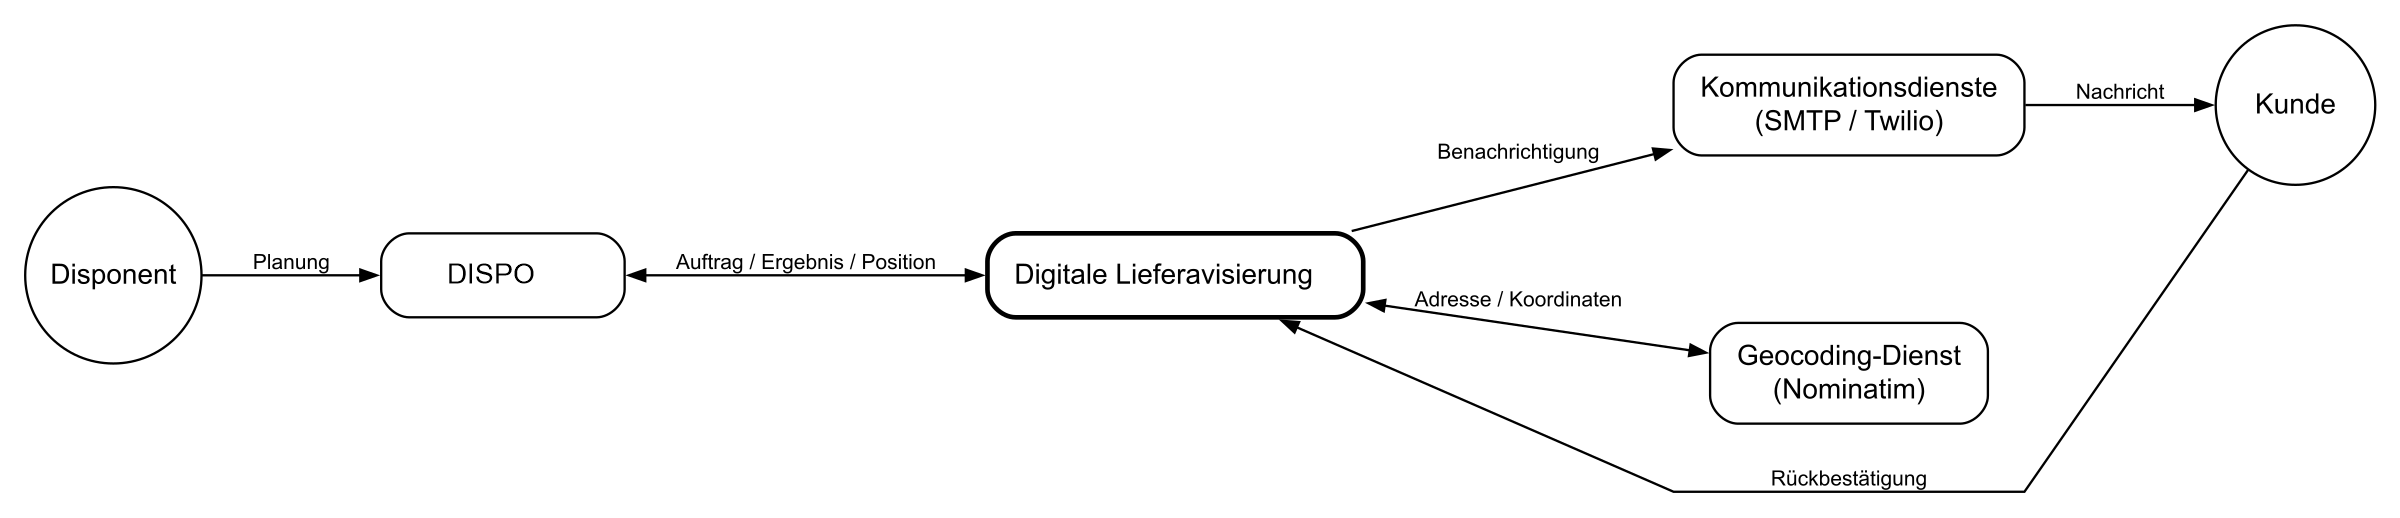
\includegraphics[
    width=\textwidth,
    keepaspectratio
  ]{figures/systemkontext.png}
  \caption{Systemkontext der digitalen Lieferavisierung}
  \label{fig:systemkontext-lieferavisierung}
\end{figure}

Damit bildet die digitale Lieferavisierung eine abgegrenzte Integrationslösung
zwischen DISPO, den beteiligten Benutzern und den externen technischen
Diensten.

\subsection{Systemkomponenten und Verantwortlichkeiten}
\label{sec:systemkomponenten-verantwortlichkeiten}

Das Webfrontend übernimmt die Benutzerinteraktion, der Avisierungsservice die
fachliche Verarbeitung und die PostgreSQL-Datenbank die dauerhafte Datenhaltung.
Der Avisierungsservice bildet das Backend der digitalen Lieferavisierung,
während das Webfrontend die Benutzeroberflächen bereitstellt.
Abbildung~\ref{fig:architekturuebersicht-lieferavisierung} zeigt ihre Einordnung
innerhalb der Systemgrenze.

\begin{figure}[htbp]
  \centering
  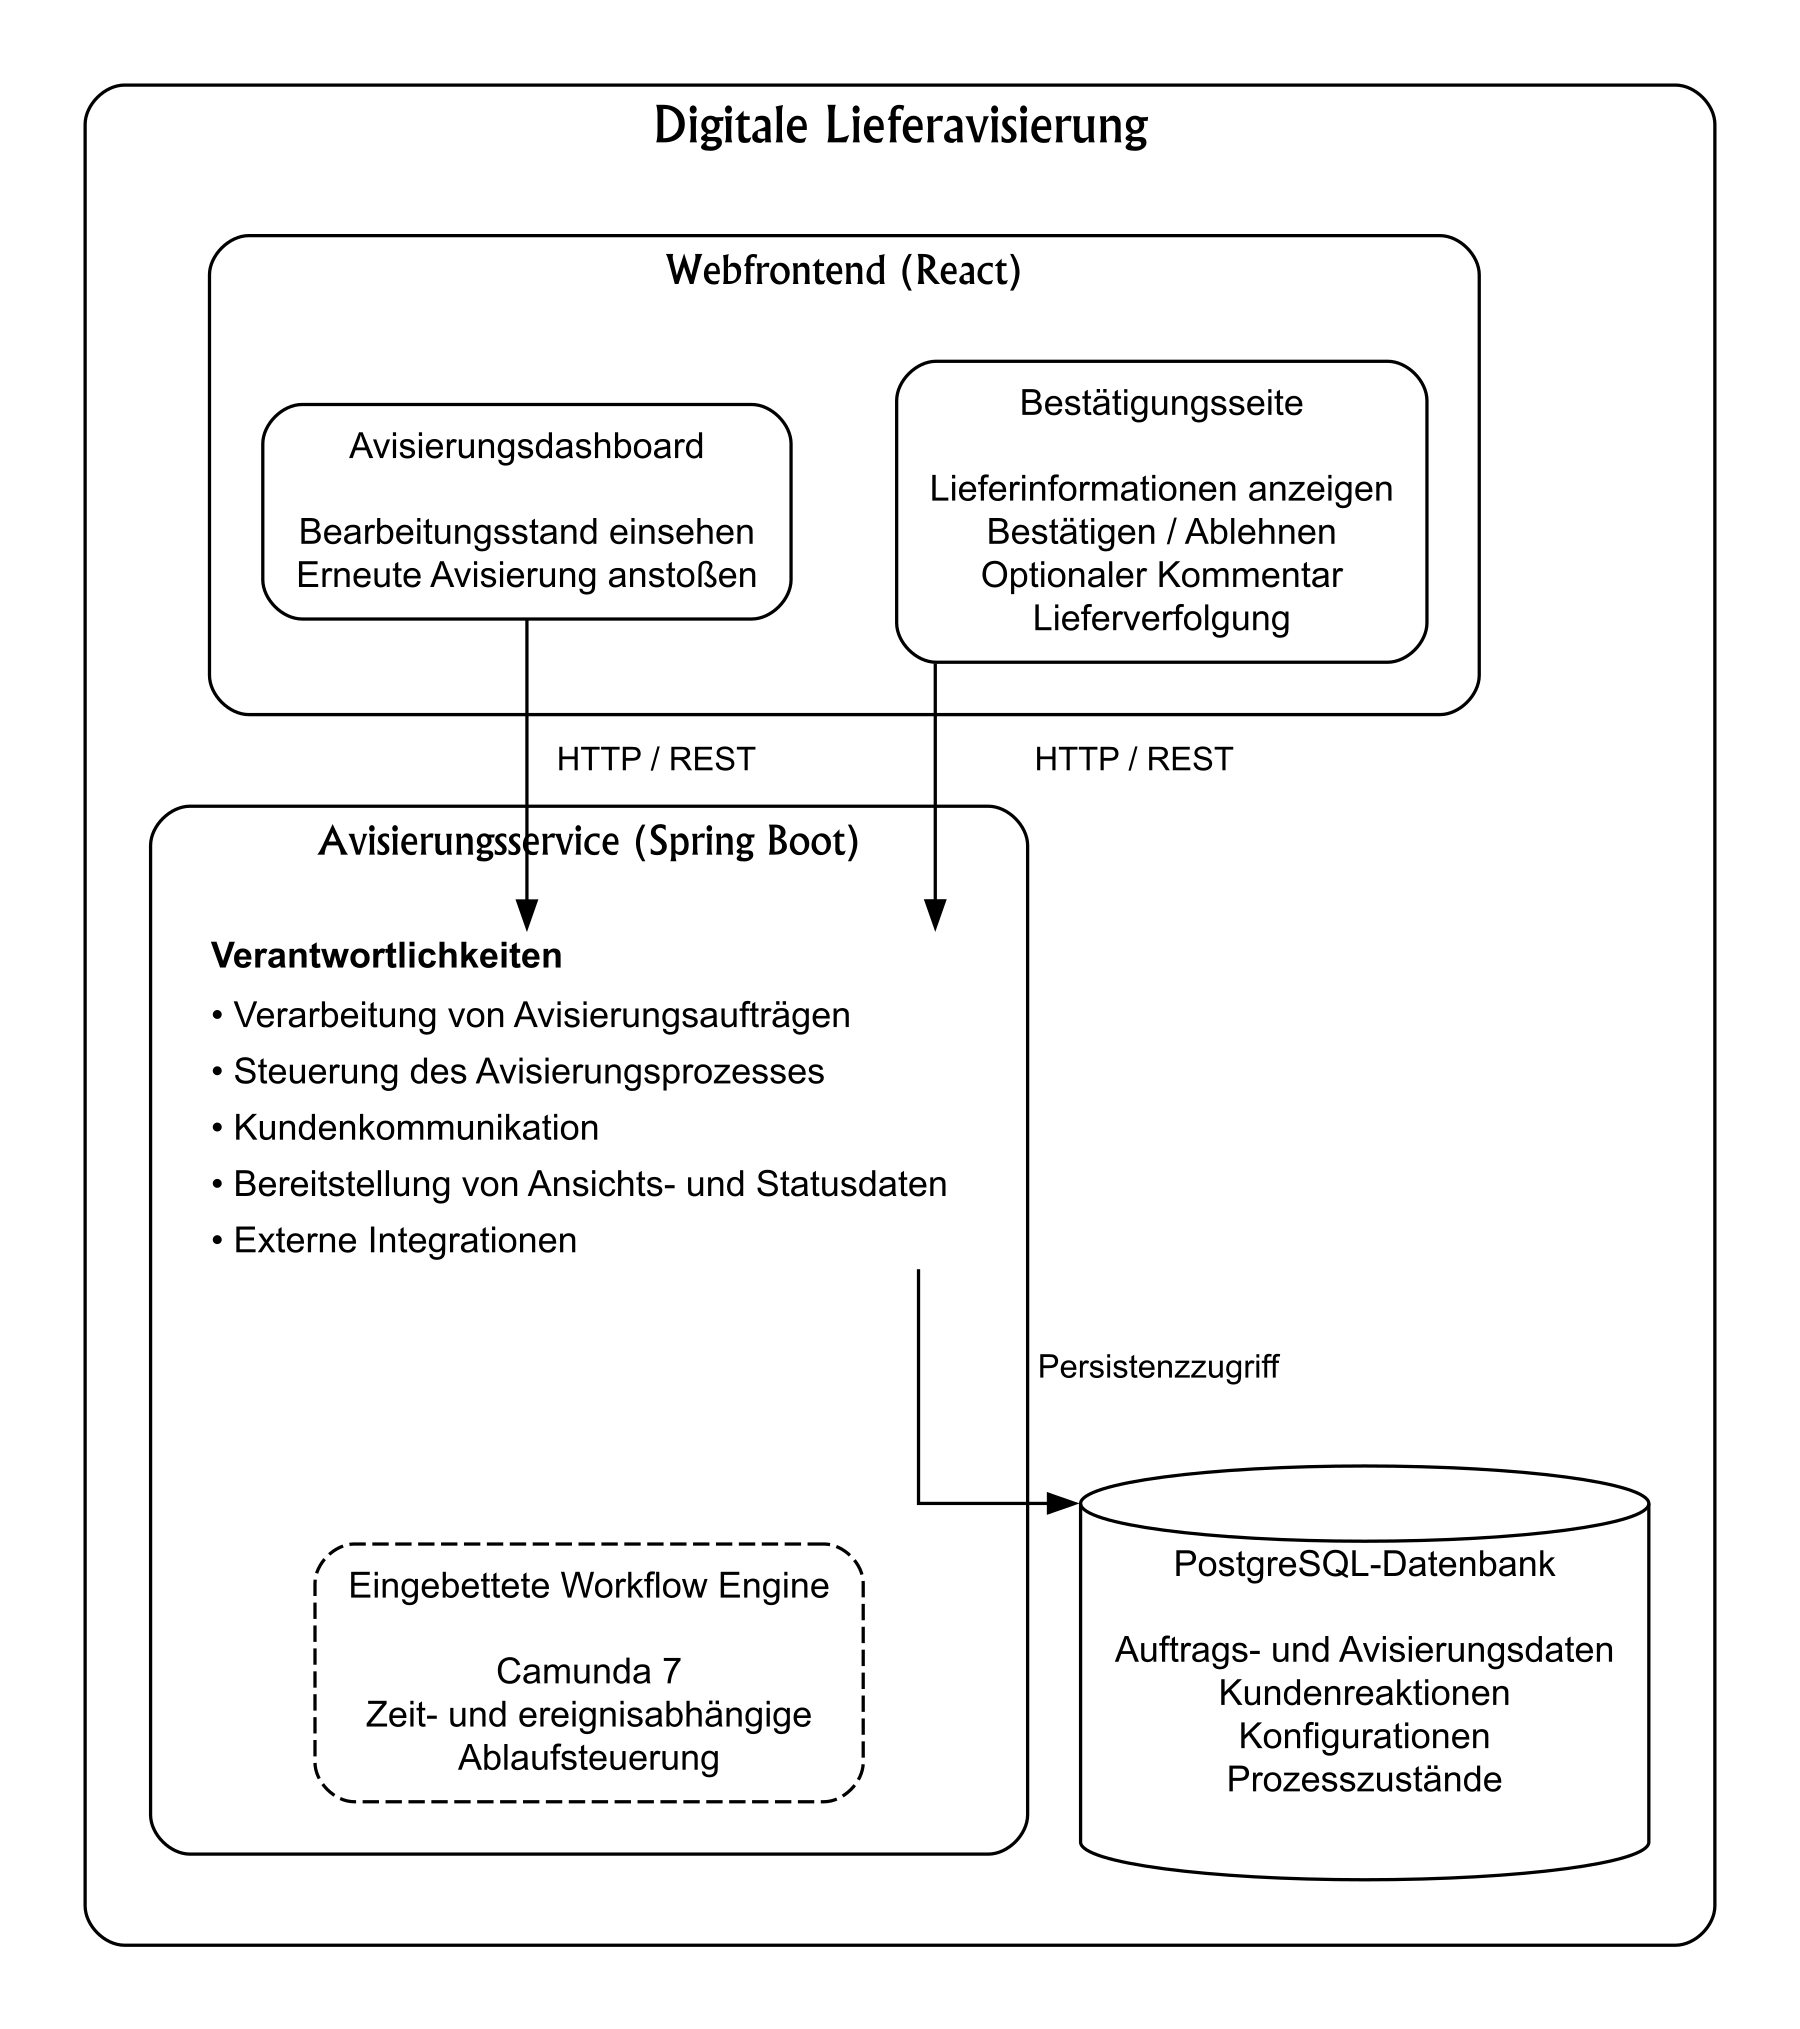
\includegraphics[
    width=0.84\textwidth,
    height=0.72\textheight,
    keepaspectratio
  ]{figures/architekturuebersicht.png}
  \caption{Architekturübersicht der digitalen Lieferavisierung}
  \label{fig:architekturuebersicht-lieferavisierung}
\end{figure}

Das \textbf{Webfrontend} ist als React-Anwendung umgesetzt und umfasst zwei
fachliche Hauptbereiche: das Avisierungsdashboard für den Disponenten sowie
die Bestätigungsseite für den Kunden. Das Avisierungsdashboard zeigt Touren,
Aufträge und Avisierungsstände, ermöglicht das Anstoßen einer erneuten
Avisierung sowie die Verwaltung der mandantenspezifischen
E-Mail-Einstellungen. Über die Bestätigungsseite können Lieferinformationen
eingesehen, Lieferzeitfenster bestätigt oder abgelehnt sowie optionale
Kommentare übermittelt werden. Für bestätigte Vorgänge steht am Liefertag
zusätzlich eine Lieferverfolgung zur Verfügung, sofern die erforderlichen
Positionsdaten verfügbar sind.

Der \textbf{Avisierungsservice} bildet die zentrale fachliche und integrative
Komponente der Lösung. Als Spring-Boot-Anwendung verarbeitet er die aus DISPO
übermittelten Avisierungsaufträge, steuert den Avisierungsprozess, verarbeitet
Kundenreaktionen, koordiniert die Kundenkommunikation und stellt die
benötigten Ansichts- und Statusdaten bereit. Darüber hinaus bindet er externe
technische Dienste an und übermittelt das resultierende Avisierungsergebnis an
DISPO. Die interne Architektur des Avisierungsservice wird in Kapitel 5
vertieft.

Der Avisierungsservice ist mandantenfähig ausgelegt. Auftragsdaten,
Dashboardzugriffe und mandantenspezifische Konfigurationen werden einem
Unternehmen zugeordnet; die konkrete Datenisolation und die zugehörigen
Sicherheitsmechanismen werden in Abschnitt~5.4 erläutert.

Die in den Avisierungsservice eingebettete \textbf{Workflow Engine Camunda 7}
übernimmt die dauerhafte Ablaufkoordination des Avisierungsprozesses. Die
konkrete Workflow-Implementierung wird in Abschnitt 5.2 erläutert.

Die \textbf{PostgreSQL-Datenbank} dient als zentraler Persistenzspeicher
innerhalb der digitalen Lieferavisierung und speichert die für den
Avisierungsprozess benötigten Anwendungs- und Prozessdaten.

\subsection{Schnittstellen und Zusammenspiel der Komponenten}
\label{sec:schnittstellen-zusammenspiel}

Im Folgenden werden die wesentlichen Kommunikationsbeziehungen innerhalb der
digitalen Lieferavisierung sowie zu den angebundenen externen Systemen
betrachtet. Abbildung~\ref{fig:schnittstellenuebersicht-lieferavisierung} zeigt
zunächst die wesentlichen Schnittstellen und Datenflussrichtungen.
Abbildung~\ref{fig:interaktionsablauf-bestaetigung} ergänzt diese statische
Sicht und zeigt exemplarisch das technische Zusammenspiel im
Avisierungsprozess.

\begin{figure}[htbp]
  \centering
  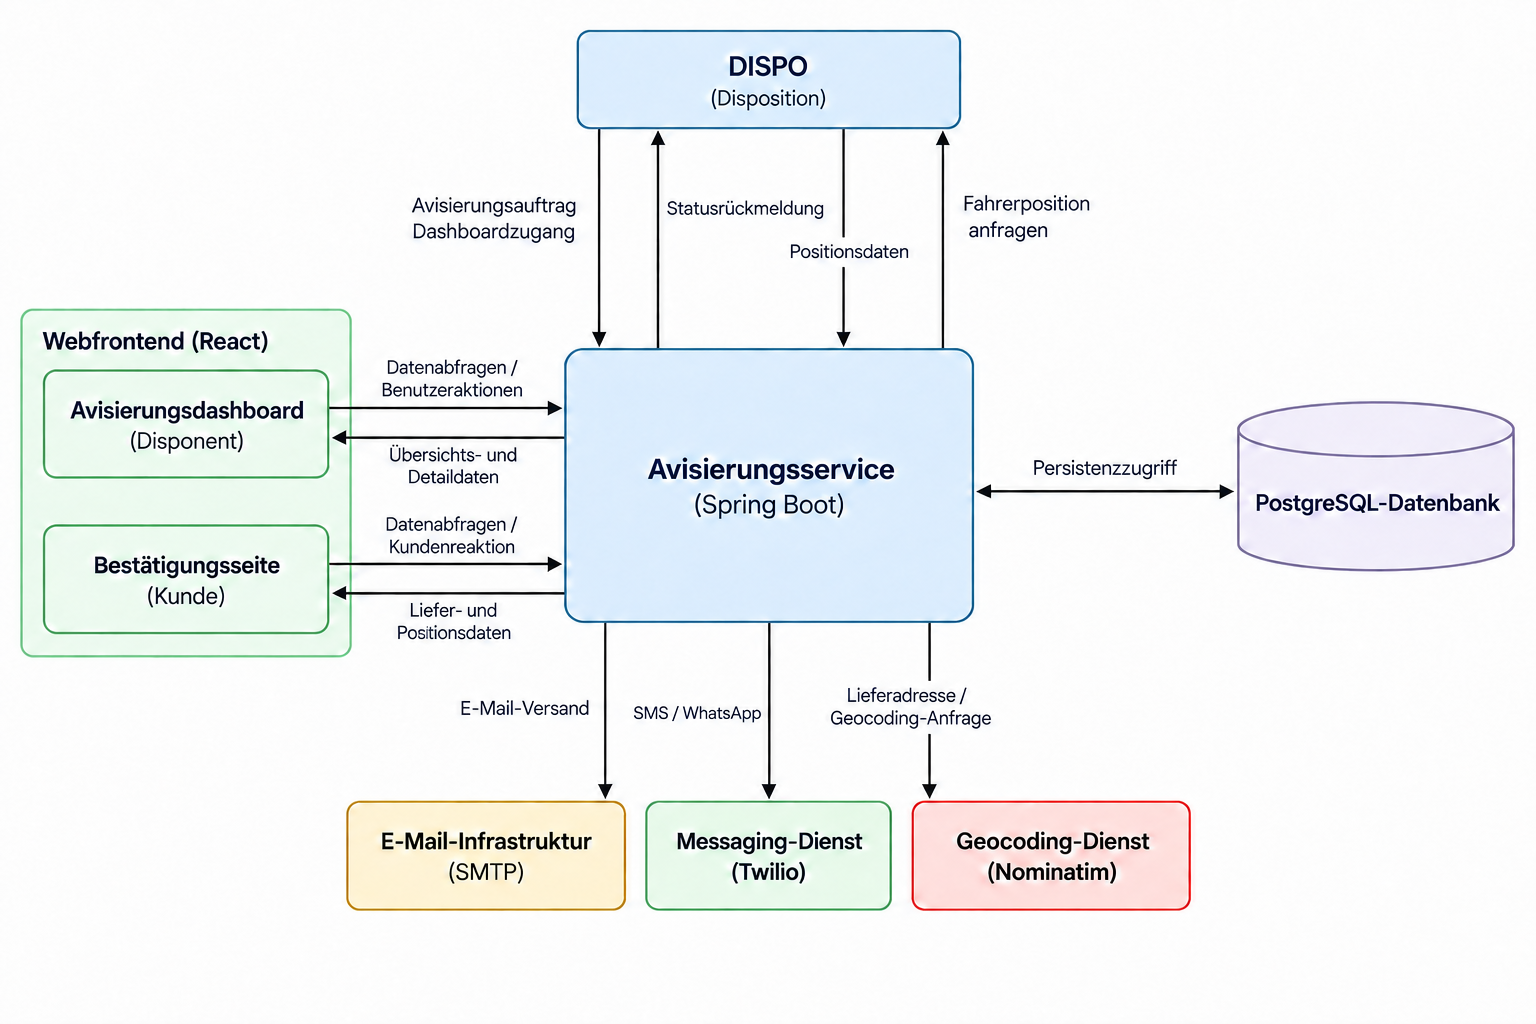
\includegraphics[
    width=\textwidth,
    height=0.68\textheight,
    keepaspectratio
  ]{figures/schnittstellenuebersicht.png}
  \caption{Wesentliche Schnittstellen der digitalen Lieferavisierung}
  \label{fig:schnittstellenuebersicht-lieferavisierung}
\end{figure}

Die Kommunikation mit DISPO umfasst mehrere fachlich unterschiedliche Vorgänge.
DISPO übermittelt Avisierungsaufträge an den Avisierungsservice und initialisiert
bei Bedarf den Zugang zum Avisierungsdashboard. Die spätere Rückmeldung eines
Avisierungsergebnisses erfolgt in Gegenrichtung. Für die
Lieferverfolgung fragt der Avisierungsservice zusätzlich die aktuelle
Fahrzeugposition bei DISPO an und erhält die zugehörigen Positionsdaten zurück.

Auch die beiden Bereiche des Webfrontends kommunizieren direkt mit dem
Avisierungsservice. Das Avisierungsdashboard übermittelt Datenabfragen und
Benutzeraktionen und erhält die benötigten Übersichts- und Detailinformationen
zurück. Der Dashboardzugang wird aus DISPO heraus initiiert; nach dem Übergang
erfolgt die weitere Kommunikation unmittelbar zwischen Webfrontend und
Avisierungsservice. Die Bestätigungsseite wird über den individuellen Link aus
der Kundenbenachrichtigung aufgerufen. Sie bezieht Liefer- und Avisierungsdaten
sowie Daten zur Lieferverfolgung vom Avisierungsservice und übermittelt die
Kundenreaktion an den Avisierungsservice.

Für die Lieferverfolgung werden Daten aus unterschiedlichen Quellen
zusammengeführt. Die Fahrzeugposition stammt aus DISPO, während die geografischen
Koordinaten des Lieferziels über den Geocoding-Dienst ermittelt werden. Hierzu
übermittelt der Avisierungsservice die Lieferadresse als Geocoding-Anfrage und
erhält die bestimmten Zielkoordinaten zurück. Weitere ausgehende Schnittstellen
dienen der Kundenkommunikation: E-Mail-Nachrichten werden über die angebundene
SMTP-Infrastruktur versendet, SMS- und WhatsApp-Nachrichten über den
Messaging-Dienst. Der Zugriff auf die PostgreSQL-Datenbank erfolgt
ausschließlich über den Avisierungsservice und dient der persistenten
Speicherung der für den Prozess benötigten fachlichen und technischen Zustände.

Abbildung~\ref{fig:interaktionsablauf-bestaetigung} zeigt ergänzend das technische Zusammenspiel
innerhalb des Avisierungsprozesses. Die Auftragsübernahme, der Aufruf
der Bestätigungsseite, die Kundenreaktion und die spätere Statusrückmeldung
an DISPO erfolgen zeitlich getrennt. Die Workflow Engine koordiniert diese
zeitlich getrennten Schritte über einen persistent verwalteten Prozesszustand;
die interne
Umsetzung wird in Abschnitt~5.2 erläutert.

\begin{figure}[htbp]
  \centering
  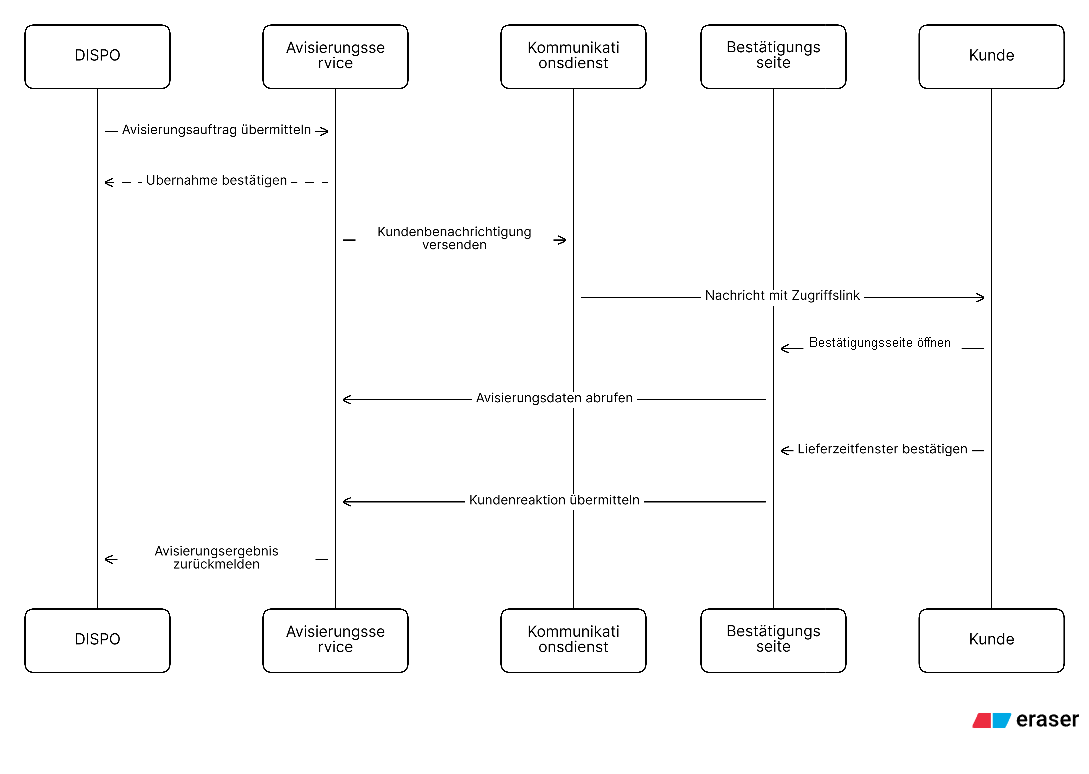
\includegraphics[
    width=\textwidth,
    height=0.70\textheight,
    keepaspectratio
  ]{figures/interaktionsablauf.png}
  \caption{Exemplarischer technischer Interaktionsablauf im Avisierungsprozess}
  \label{fig:interaktionsablauf-bestaetigung}
\end{figure}

\clearpage

\input{kapitel/05-avisierungsservice}
\section{Frontend -- Konzeption und Implementierung}


% -------------------------------------------------
% 6.1
% -------------------------------------------------

\subsection{Einordnung des Frontends in das Gesamtsystem}


% -------------------------------------------------
% 6.2
% -------------------------------------------------

\subsection{Frontend-Architektur und technische Grundlagen}

\subsubsection{Technologieauswahl}

\subsubsection{Seiten-, Komponenten- und Routingstruktur}

\subsubsection{API-Anbindung und Zustandsverwaltung}

\subsubsection{Responsive Design und wiederverwendbare UI-Komponenten}


% -------------------------------------------------
% 6.3
% -------------------------------------------------

\subsection{Avisierungsdashboard}

\subsubsection{Geschützter Dashboard-Zugang}

\subsubsection{Tourübersicht und Statusdarstellung}

\subsubsection{Suche, Filterung und Paginierung}


% -------------------------------------------------
% 6.4
% -------------------------------------------------

\subsection{Auftragsdetailansicht und erneute Avisierung}

\subsubsection{Auftragsdaten und Avisierungshistorie}

\subsubsection{Erneute Avisierung, Validierung und Fehlerrückmeldung}


% -------------------------------------------------
% 6.5
% -------------------------------------------------

\subsection{Bestätigungsseite für Kunden}

\subsubsection{Tokenbasierter Zugriff und Lieferinformationen}

\subsubsection{Bestätigung, Ablehnung und Kundenkommentar}

\subsubsection{Abgeschlossene, abgelaufene und fehlerhafte Anfragen}


% -------------------------------------------------
% 6.6
% -------------------------------------------------

\subsection{Live-Tracking}

\subsubsection{Verfügbarkeit und Datenfluss}

\subsubsection{Karten- und Positionsdarstellung}

\subsubsection{Aktualisierung und Fehlerbehandlung}

\section{Test und Validierung}

\subsection{Teststrategie und Testumgebung}

Die Validierung erfolgte schrittweise entlang der zentralen
Anwendungsfälle. Zunächst wurden einzelne Komponenten isoliert
überprüft, anschließend das Zusammenspiel von Frontend,
Backend, Workflow Engine und Kommunikationskanälen getestet.

Ein besonderer Fokus lag dabei auf den Übergängen zwischen den
Systemkomponenten, da dort fachliche Fehler oder inkonsistente
Status besonders wahrscheinlich sind.

\subsubsection{Testziele, Testebenen und Auswahl der Prüfschwerpunkte}

\subsubsection{Testwerkzeuge und reproduzierbare Testumgebung}

\subsection{Validierung des Avisierungsservice}

\subsubsection{Domänen- und Anwendungslogik}

\subsubsection{REST-Verträge, Eingabevalidierung und Fehlerantworten}

\subsubsection{Authentifizierung, Sitzungsverwaltung und Mandantenisolation}

\subsubsection{Persistenz- und Abfragemodell}

\subsubsection{Workflow-, Wiederholungs- und Nebenläufigkeitsszenarien}

\subsubsection{Ausgehende Schnittstellen und Rückkanäle}

\subsection{End-to-End-Tests}

Die End-to-End-Tests prüfen die zentralen Benutzerabläufe der
Kundenbestätigung, des Dispositions-Dashboards und der
Lieferverfolgung über Frontend, Backend, E-Mail-Versand und
DISPO-Rückmeldung hinweg. Sie werden mit Playwright im
Chromium-Browser ausgeführt und befinden sich im Verzeichnis
\texttt{frontend/tests}.

\subsubsection{Einordnung der Szenariogruppen}

Die Teststruktur orientiert sich an fachlichen Benutzerabläufen
und nicht an einzelnen Frontend-Komponenten. Die Szenarien sind
in die Bereiche Kundenbestätigung, Dispositions-Dashboard und
Lieferverfolgung gegliedert.

Die Szenarien zur Kundenbestätigung umfassen den Versand und
Inhalt der Bestätigungs-E-Mail, den Zugriff auf die Kundenseite,
die Anzeige der Lieferdaten sowie die Bestätigung oder Ablehnung
eines Liefertermins. Zusätzlich werden ungültige
Bestätigungstoken, optionale Kundenkommentare und die Persistenz
bereits abgegebener Antworten geprüft. Die
Dashboard-Szenarien prüfen den geschützten Zugang, die
Tourenübersicht, die Suche und Filterung, die Auftragsdetails,
die Avisierungshistorie und die Auswahl des Kommunikationskanals
für eine erneute Avisierung. Die Tracking-Szenarien prüfen die
Verfügbarkeit und Aktualisierung der Lieferverfolgung.

\subsubsection{Testumgebung und technische Struktur}

Die Testsuite enthält insgesamt 29 Playwright-Tests. Davon
bilden 28 Tests fachliche End-to-End-Szenarien ab. Ein
zusätzlicher Setup-Test prüft vor der Ausführung die
Erreichbarkeit der benötigten Dienste.

Die fachlichen Tests befinden sich in den Verzeichnissen
\texttt{frontend/tests/confirmation},
\texttt{frontend/tests/dashboard} und
\texttt{frontend/tests/tracking}.

Die Tests zur Kundenbestätigung sind auf folgende Dateien
verteilt:

\begin{itemize}
    \item \texttt{email.spec.ts} für den Versand und Inhalt der
    Bestätigungs-E-Mail
    \item \texttt{page.spec.ts} für die Anzeige der Kundenseite
    und das Verhalten bei ungültigen Bestätigungstoken
    \item \texttt{response.spec.ts} für Bestätigung, Ablehnung,
    Kundenkommentare, DISPO-Rückmeldungen und persistierte
    Abschlusszustände
\end{itemize}

Die Tests des Dispositions-Dashboards befinden sich in folgenden
Dateien:

\begin{itemize}
    \item \texttt{authentication.spec.ts} für den gültigen und
    ungültigen Dashboard-Zugang
    \item \texttt{overview.spec.ts} für die Tourenübersicht,
    Statusanzahlen, Suche, Filterung und Pagination,
    \item \texttt{order-detail.spec.ts} für Auftragsdetails,
    Anfragehistorie, Kundenreaktionen, Resend-Berechtigung und
    Kanalauswahl
    \item \texttt{settings.spec.ts} für das Laden und Testen der
    E-Mail- und SMTP-Einstellungen
\end{itemize}

Die Tests zur Lieferverfolgung befinden sich in
\texttt{frontend/tests/tracking/tracking.spec.ts}. Sie prüfen
die Tracking-Karte, die Fahrzeug- und Zielmarkierung, die
Anzeige der Zieladresse, die Verfügbarkeit vor dem Liefertag
und die Aktualisierung der Fahrerposition.

Wiederverwendbare technische Abläufe befinden sich unter
\texttt{frontend/tests/helpers}. Dazu gehören das Erzeugen
eindeutiger Testaufträge, das Auslesen von E-Mails aus Mailpit,
das Öffnen einer authentifizierten Dashboard-Sitzung, die
Prüfung von DISPO-Rückmeldungen und die Vorbereitung bestätigter
Aufträge für Tracking-Szenarien.

Vor den fachlichen Tests führt Playwright den Setup-Test
\texttt{setup/services.setup.ts} aus. Dieser prüft einmalig die
Erreichbarkeit von Backend, Mailpit und DISPO-Mock. Die
Prüfungen verwenden Polling, damit die Testausführung auf den
Start der benötigten Docker-Dienste warten kann.

Dynamisch erzeugte Testaufträge erhalten mit
\texttt{randomUUID()} eindeutige Auftragsnummern und
E-Mail-Adressen. Die Dashboard-Tests verwenden vorbereitete
\texttt{DEMO}-Seed-Daten. Playwright verändert dabei keine
Datenbankzustände direkt.

\subsubsection{Versand und Bereitstellung der Anfrage}

Zur Prüfung des Versandablaufs wird über die geschützte
DISPO-Schnittstelle eine Bestätigungsanfrage für einen
eindeutigen Testauftrag erzeugt. Die dadurch ausgelöste
Bestätigungs-E-Mail wird über den konfigurierten SMTP-Versand
an Mailpit übermittelt. Dort wartet der Test auf den Eingang
der Nachricht.

Anschließend wird überprüft, ob die E-Mail den Kundennamen, die
Lieferadresse, das Produkt, die Bestellmenge, das
Lieferzeitfenster, den Preis und den personalisierten
Bestätigungslink enthält.

Damit bildet das Szenario den systemübergreifenden Ablauf von
der Anlage eines Avisierungsauftrags bis zur Bereitstellung
eines für den Kunden nutzbaren Bestätigungslinks ab. Bewertet
wird dabei die tatsächlich in Mailpit eingegangene Nachricht.

\subsubsection{Kundenzugriff und Anzeige der Lieferdaten}

Nach dem Öffnen des Bestätigungslinks wird geprüft, ob die
Bestätigungsseite alle für die Kundenentscheidung erforderlichen
Informationen anzeigt. Dazu gehören Kundenname, Lieferadresse,
Produkt, Bestellmenge, Preis sowie Beginn und Ende des
Lieferzeitfensters.

Zusätzlich wird geprüft, wie die Anwendung auf ein unbekanntes
Bestätigungstoken reagiert. Sie zeigt in diesem Fall eine
verständliche Fehlermeldung an und bietet keine Möglichkeit,
den Liefertermin zu bestätigen oder abzulehnen.

\subsubsection{Kundenreaktion und DISPO-Rückmeldung}

Die Bestätigung und die Ablehnung eines Liefertermins werden als
getrennte E2E-Szenarien geprüft.

Nach der Bestätigung muss die Anwendung eine sichtbare
Erfolgsmeldung anzeigen. Zusätzlich wird geprüft, ob der
DISPO-Mock eine Rückmeldung mit der externen Auftragsnummer und
dem Status \texttt{CONFIRMED} erhält.

Ein weiterer Test prüft die Übermittlung einer optionalen
Kundennachricht im Bestätigungsablauf. Der eingegebene Kommentar
muss gemeinsam mit der \texttt{CONFIRMED}-Rückmeldung an den
DISPO-Mock übertragen werden. Da für Bestätigung und Ablehnung
dasselbe Kommentarfeld und derselbe Übertragungsweg verwendet
werden, wird die Kommentarübermittlung nur einmal im
Bestätigungsablauf geprüft.

Nach der Ablehnung muss die Anwendung ebenfalls eine sichtbare
Rückmeldung anzeigen. Der DISPO-Mock muss dabei den Status
\texttt{REJECTED} für die entsprechende externe Auftragsnummer
erhalten.

Die Persistenz beider Abschlusszustände wird durch das erneute
Öffnen des Bestätigungslinks geprüft. Der zuvor erreichte Status
muss weiterhin angezeigt werden, während die Buttons zum
Bestätigen und Ablehnen nicht mehr verfügbar sind. Im
abgelehnten Zustand darf außerdem keine Tracking-Karte
angezeigt werden.

\subsubsection{Dashboard-Zugang}

Für den Dashboard-Zugang fordert der Test mithilfe eines gültigen
API-Schlüssels über die geschützte Backend-Schnittstelle einen
Dashboard-Zugangslink an. Nach dem Öffnen dieses Links im Browser
prüft der Test den Aufbau einer authentifizierten
Dashboard-Sitzung, die Weiterleitung zum Dispositions-Dashboard
und die Anzeige der Tourenübersicht.

Ein weiterer Test ruft die Anwendung mit einem ungültigen
Zugangscode auf. In diesem Fall darf das Dashboard nicht
angezeigt werden. Stattdessen muss die Anwendung eine
verständliche Fehlermeldung ausgeben.

\subsubsection{Tourenübersicht, Suche und Filterung}

In der Tourenübersicht werden die verfügbaren Touren, die
zugehörigen Aufträge und die aggregierten Statusanzahlen
kontrolliert. Dabei werden bestätigte, abgelehnte und noch
unbeantwortete Aufträge berücksichtigt.

Die globale Suche wird in getrennten Szenarien mit einem
Kundennamen, einer Auftragsnummer und einer Lieferadresse
ausgeführt. Dabei wird jeweils geprüft, ob der gesuchte Auftrag
angezeigt und ein nicht passender Auftrag aus der Ergebnisliste
entfernt wird.

Zusätzlich wird die kombinierte Filterung nach Tournummer und
Bestätigungsstatus geprüft. Der Pagination-Test wechselt auf die
zweite Ergebnisseite, kontrolliert den dafür ausgeführten
Backend-Aufruf und prüft die Anzeige der dort enthaltenen
Ergebnisse.

\subsubsection{Auftragsdetails und erneute Avisierung}

Die Auftragsdetailseite zeigt die Stammdaten des Auftrags, den
aktuellen Status und die aktuelle Bestätigungsanfrage. Die
E2E-Tests prüfen unter anderem die Auftragsnummer, den
Kundennamen, die E-Mail-Adresse, die Lieferadresse, das Fahrzeug,
die Bestellmenge und den Kommunikationskanal.

Darüber hinaus wird die Avisierungshistorie geprüft. Historische
Anfragen mit den Zuständen \texttt{REJECTED} und
\texttt{NO\_RESPONSE} sowie gespeicherte Kundenkommentare müssen
auf der Detailseite sichtbar sein.

Die Verfügbarkeit der erneuten Avisierung hängt vom aktuellen
Status ab. Für einen bereits bestätigten Auftrag muss der Button
\glqq Erneut senden\grqq deaktiviert sein. Für einen Auftrag mit
dem Status \texttt{NO\_RESPONSE} muss der Button dagegen
aktiviert sein.

Für eine zulässige erneute Avisierung wird die Auswahl der
Kommunikationskanäle E-Mail, SMS und WhatsApp geprüft. Nach der
Auswahl eines Kanals muss die vorherige Auswahl aufgehoben und
der aktive Kanal über das Attribut \texttt{aria-pressed}
zugänglich gekennzeichnet werden. Der Button zum erneuten Senden
muss dabei aktiviert bleiben.

Der Versand wird im E2E-Test nicht ausgelöst, da die
Dashboard-Tests gemeinsam verwendete \texttt{DEMO}-Seed-Daten
nutzen. Eine erneute Avisierung würde die aktuelle Anfrage und
ihre Historie verändern und dadurch die Wiederholbarkeit der
Tests beeinträchtigen.

Für SMS und WhatsApp wird ausschließlich die Auswahl in der
Benutzeroberfläche geprüft. Ein tatsächlicher Versand über
Twilio erfolgt nicht, um kostenpflichtige Nachrichten an externe
Empfänger und eine Abhängigkeit von der Verfügbarkeit eines
Drittdienstes zu vermeiden.

\subsubsection{E-Mail- und SMTP-Einstellungen}

Die E-Mail-Einstellungen des Dashboards werden in drei
Szenarien geprüft.

Zunächst wird kontrolliert, ob die gespeicherten
SMTP-Einstellungen vom Backend geladen und in der
Benutzeroberfläche dargestellt werden.

Anschließend wird über den Button
\glqq Verbindung testen\grqq{} geprüft, ob das Backend die
gespeicherte SMTP-Konfiguration erfolgreich verwenden kann.
Nach erfolgreichem Abschluss muss eine entsprechende Meldung
angezeigt werden.

Der dritte Test versendet eine SMTP-Test-E-Mail. Neben der
sichtbaren Erfolgsmeldung wird geprüft, ob Mailpit tatsächlich
eine neue Nachricht mit dem erwarteten Betreff erhalten hat.

\subsubsection{Lieferverfolgung und Tracking-Verfügbarkeit}

Für bestätigte Lieferungen am Liefertag wird geprüft, ob die
Live-Tracking-Ansicht verfügbar ist. Die Tracking-Schnittstellen
müssen gültige Ziel- und Fahrerkoordinaten liefern. In der
Benutzeroberfläche müssen die Tracking-Karte sowie die
Fahrzeug- und Zielmarkierung sichtbar sein.

Ein weiteres Szenario prüft, ob die Lieferadresse als
Zieladresse angezeigt wird und die Zielmarkierung auf der Karte
sichtbar ist.

Bei einer bestätigten Lieferung mit einem zukünftigen
Lieferdatum meldet die Tracking-Schnittstelle, dass die
Lieferverfolgung noch nicht verfügbar ist, und liefert keine
Zielkoordinaten. Die Anwendung zeigt daher weder die
Tracking-Karte noch die Fahrzeug- und Zielmarkierung an.
Stattdessen wird der Kunde darauf hingewiesen, dass die
Tracking-Informationen erst am Liefertag verfügbar sind.

Abschließend wird die Aktualisierung der Fahrerposition über den
Button \glqq Aktualisieren\grqq{} geprüft. Dabei müssen neue
Fahrerkoordinaten geladen und der angezeigte Lieferstatus
beziehungsweise die verbleibende Entfernung aktualisiert
werden. Die Karte sowie die Fahrzeug- und Zielmarkierung müssen
weiterhin sichtbar bleiben.

\section{Projektmanagement und Projektreflexion}

\subsection{Projektmanagement}

\subsubsection{Projektphasen}

Das Projekt wurde in klar abgegrenzte Phasen unterteilt, um
Analyse, Konzeption, Umsetzung und Validierung strukturiert
durchführen zu können. Die Übergänge zwischen den Phasen waren
teilweise iterativ, da Erkenntnisse aus der Implementierung
wieder in die Ausgestaltung des SOLL-Prozesses eingeflossen
sind.

\begin{table}[H]
\centering
\begin{tabular}{p{5cm}p{4cm}p{3cm}}
\toprule
Phase & Zeitraum & Status \\
\midrule
Analyse und Anforderungsabstimmung & xx.xx - xx.xx & abgeschlossen \\
Architektur und Prozessmodellierung & xx.xx - xx.xx & abgeschlossen \\
Implementierung & xx.xx - xx.xx & abgeschlossen \\
Integration und Test & xx.xx - xx.xx & abgeschlossen \\
Abschluss und Ergebnisaufbereitung & xx.xx - xx.xx & abgeschlossen \\
\bottomrule
\end{tabular}
\end{table}

\subsubsection{Projektplan}

Der Projektplan diente als gemeinsame Orientierung für
inhaltliche Meilensteine, Abstimmungstermine und die
Reihenfolge der Umsetzung. Besonders hilfreich war die frühe
Sichtbarkeit von Abhängigkeiten zwischen Prozessmodell,
Schnittstellen und Benutzeroberfläche.

\begin{figure}[H]
\centering

\includegraphics[width=\textwidth]{../Projektplan/assets/projectplan.png}
\caption{Projektplan}
\end{figure}

\subsubsection{Projektaufwand}

Der dokumentierte Aufwand verteilt sich auf Analyse,
Konzeption, Implementierung, Test und Abstimmung mit dem
Auftraggeber. Die Tabelle dient als Beispielstruktur zur
Erfassung der geleisteten Stunden und kann mit den tatsächlichen
Projektdaten vervollständigt werden.

\begin{longtable}{p{2cm}p{3cm}p{5cm}p{2cm}}
\toprule
Datum & Person & Tätigkeit & Stunden \\
\midrule
xx.xx.2026 & Name 1 & Anforderungsanalyse und Recherche & 4 \\
\midrule
xx.xx.2026 & Name 2 & Backend-Implementierung & 6 \\
\midrule
xx.xx.2026 & Name 3 & BPMN-Modellierung und Camunda-Integration & 5 \\
\midrule
xx.xx.2026 & Name 1 & Frontend-Umsetzung und UI-Anpassungen & 5 \\
\midrule
xx.xx.2026 & Team & Integrationstest und Ergebnisabstimmung & 4 \\
\bottomrule
\end{longtable}

\subsection{Projektreflexion}

\subsubsection{Herausforderungen}

Herausfordernd war insbesondere die Abstimmung an den
Schnittstellen zwischen fachlicher Prozessbeschreibung und
technischer Umsetzung. Bereits kleine Unklarheiten bei
Statusübergängen oder Rückmeldewegen hatten direkte
Auswirkungen auf mehrere Systemkomponenten.

Auch die Konsistenz zwischen Benutzerführung, Datenmodell und
Workflowlogik erforderte wiederholte Abstimmungen.

\subsubsection{Lessons Learned}

Für vergleichbare Projekte empfiehlt es sich, Statusmodelle,
Ereignisse und Verantwortlichkeiten frühzeitig gemeinsam zu
definieren und schriftlich festzuhalten. Darüber hinaus hat
sich gezeigt, dass ein visuelles Prozessmodell in Kombination
mit einer frühen technischen Teilimplementierung sehr hilfreich
ist, um Missverständnisse schnell sichtbar zu machen.

\section{Projektrgebnisse}

\subsection{Gesamtergebnis}

Die Projektarbeit führte zu einem konsistenten Prototypen, der
die wesentlichen Anforderungen des definierten SOLL-Prozesses
abbildet.

\begin{itemize}
    \item Funktionsfähiger Prototyp
    \item Frontend-Backend-Kommunikation
    \item Automatisierte Kommunikation über verschiedene Kanäle
    \item Digitale Rückbestätigung von Lieferterminen
    \item Statusverwaltung
    \item Workflow-Steuerung
    \item Avisierungsdashboard für die Disposition
    \item Bestätigungsseite für Kunden
    \item Lieferverfolgung bzw. Fahrerkartenansicht
\end{itemize}

\subsection{Grenzen des Projektergebnisses}

\subsection{Fazit und Ausblick}
Das Projekt konnte sowohl aus technischer als auch aus
organisatorischer Sicht erfolgreich abgeschlossen werden. Neben
dem entwickelten Prototypen entstand eine belastbare Grundlage
für die weitere fachliche und technische Ausarbeitung des
Systems.

Die Kombination aus Prozessmodellierung, Webanwendung und
automatisierter Kommunikation erwies sich als geeigneter Ansatz
für die Digitalisierung des betrachteten Anwendungsfalls.

\section{Nutzung von Künstlicher Intelligenz}

Für die Projektdokumentation und die technische Ausarbeitung wurden verschiedene KI-gestützte Arbeitsschritte durchgeführt. Dabei standen vor allem die Recherche, die Strukturierung von Ideen und die sprachliche Überarbeitung im Vordergrund.

Im Bereich der Softwareentwicklung wurden Bezeichnungen im Code überprüft und verbessert. Dabei ging es vor allem um verständliche Namen für Klassen, Methoden, Variablen und fachliche Begriffe. Dadurch sollten die Struktur des Codes und die Lesbarkeit für alle Projektmitglieder verbessert werden.

Bei der Planung der Kundenkommunikation wurden mögliche Kommunikationswege wie SMS oder WhatsApp miteinander verglichen. Dabei wurde betrachtet, wie Kunden über geplante Liefertermine informiert werden können, wie eine Rückmeldung zum Termin erfolgen könnte und welche technischen Anforderungen sich daraus für das System ergeben.

Für das Thema Live-Tracking wurden grundlegende Umsetzungsmöglichkeiten untersucht. Dazu gehörten Überlegungen dazu, welche Standortinformationen für eine Lieferung relevant sind, wie diese Daten an das Backend übertragen werden können und wie eine verständliche Darstellung im Frontend aussehen könnte.

Auch einzelne Abschnitte der Dokumentation wurden sprachlich überarbeitet. Dabei wurden Formulierungen verständlicher gemacht, Inhalte besser gegliedert und technische Beschreibungen an den Stil einer Projektdokumentation angepasst.

Alle Ergebnisse wurden anschließend von der Projektgruppe geprüft, angepasst und in den jeweiligen Arbeitsbereich eingeordnet. Die fachlichen Entscheidungen, die technische Umsetzung und die finale Ausarbeitung erfolgten durch die Projektmitglieder.
\input{kapitel/11-hilfsmittel}

\clearpage
\printbibliography[
  heading=bibintoc,
  title={Literaturverzeichnis}
]

\end{document}
